%%%%%%%%%%%%%%%%%%%%%%%%%%%%%%%%%%%%%%%%%
% University/School Laboratory Report
% LaTeX Template
% Version 3.1 (25/3/14)
%
% This template has been downloaded from:
% http://www.LaTeXTemplates.com
%
% Original author:
% Linux and Unix Users Group at Virginia Tech Wiki 
% (https://vtluug.org/wiki/Example_LaTeX_chem_lab_report)
%
% License:
% CC BY-NC-SA 3.0 (http://creativecommons.org/licenses/by-nc-sa/3.0/)
%
%%%%%%%%%%%%%%%%%%%%%%%%%%%%%%%%%%%%%%%%%

%----------------------------------------------------------------------------------------
%	PACKAGES AND DOCUMENT CONFIGURATIONS
%----------------------------------------------------------------------------------------

\documentclass{article}

\usepackage[version=3]{mhchem} % Package for chemical equation typesetting
%\usepackage{siunitx} % Provides the \SI{}{} and \si{} command for typesetting SI units
\usepackage{graphicx} % Required for the inclusion of images
\usepackage{natbib} % Required to change bibliography style to APA
\usepackage{amsmath} % Required for some math elements 
\usepackage{hyperref}
 \usepackage{pdflscape}
\usepackage[a4paper,margin=0.5in]{geometry}
\setlength\parindent{0pt} % Removes all indentation from paragraphs

\renewcommand{\labelenumi}{\alph{enumi}.} % Make numbering in the enumerate environment by letter rather than number (e.g. section 6)

%\usepackage{times} % Uncomment to use the Times New Roman font

%----------------------------------------------------------------------------------------
%	DOCUMENT INFORMATION
%----------------------------------------------------------------------------------------

\title{Gate Detection} % Title

\author{Philipp \textsc{Duernay}} % Author name

\date{\today} % Date for the report

\begin{document}
\maketitle
% If you wish to include an abstract, uncomment the lines below
% \begin{abstract}
% Abstract text
% \end{abstract}

%----------------------------------------------------------------------------------------
%	SECTION 1
%----------------------------------------------------------------------------------------

\section{Recap}
In the last meeting from 06.06.2018 several next steps were defined:
\begin{itemize}
	\item Finish two stage approach
	\item Study effect of fast architectures (mobilenet, shufflenet, wide-residual net)
\end{itemize}


\section{Fast architectures}

Last time I mentioned that there are fast architectures but that those are not implemented in darknet, which makes them difficult to use. However, there is one structure which can be used and those are the so called bottlenecks. The principle is displayed in Fig. \ref{fig:bottleneck}. \autoref{tab:bottleneck} shows time measurements for an input volume of 13x13x64 on the Jevois.

\begin{figure}[htbp]
		\centering
	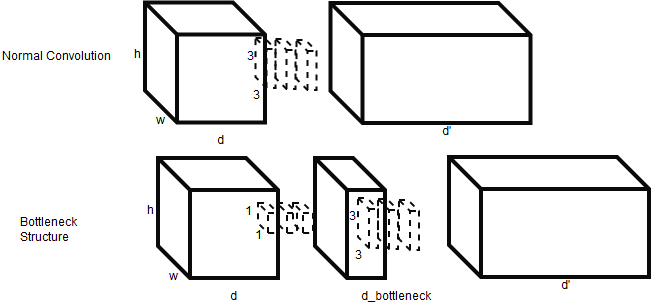
\includegraphics[width=0.5\linewidth]{bottleneck}
	\label{fig:bottleneck}
	\caption{Instead of directly applying a 3x3xd convolution to the input volume, first a 1x1xd convolution is used to reduce the number of channels. That way the total number of computations is reduced. }
\end{figure}

\begin{table}[htbp]

	\caption{Inference Time Bottleneck on JeVois. 0.5 is the "compression" factor. So in this case the 64 input volume is compressed to 32 channels.}
	\begin{center}
		\begin{tabular}{|r|r|r|}
			\hline
			\multicolumn{1}{|l|}{\textbf{n\_filters (input vol 13x13x64)}} & \multicolumn{1}{l|}{\textbf{Standard Conv}} & \multicolumn{1}{l|}{\textbf{Bottleneck 0.5}} \\ \hline
			64 & 2.3 & 2 \\ \hline
			128 & 4.09 & 2.87 \\ \hline
			256 & 7.48 & 5.41 \\ \hline
		\end{tabular}
	\end{center}
	\label{tab:bottleneck}
\end{table}

\begin{table}[htbp]
	\caption{Inference Time Strides vs Pooling on JeVois}
	\begin{center}
		\begin{tabular}{|l|r|r|}
			\hline
			\textbf{Input + Filter} & \multicolumn{1}{l|}{\textbf{(2,2) Strides}} & \multicolumn{1}{l|}{\textbf{(1,1) Stride + MaxPool}} \\ \hline
			\textit{kernel6x6} & \multicolumn{1}{l|}{} & \multicolumn{1}{l|}{} \\ \hline
			208x208 & 35.6 & 144.1 \\ \hline
			104x104 & 9.6 & 37 \\ \hline
			52x52 & 2.6 & 9.7 \\ \hline
			& \multicolumn{1}{l|}{} & \multicolumn{1}{l|}{} \\ \hline
			\textit{kernel3x3} & \multicolumn{1}{l|}{} & \multicolumn{1}{l|}{} \\ \hline
			208x208 & 15.6 & 70.13 \\ \hline
			104x104 & 3.8 & 17.9 \\ \hline
			52x52 & 1.14 & 4.22 \\ \hline
		\end{tabular}
	\end{center}
	\label{tab:strides}
\end{table}

Additionally, I experimented with larger strides to reduce the computations. \autoref{tab:strides} shows time measurements on the JeVois for two different kernels. We can see how the time drops by factor of 4 when applying 2,2 strides, which corresponds to the number of computations we save. Additionally we save the pooling. This led to the different models displayed in Fig. \ref{fig:pr}.

We see again how reducing the performance has almost no effect on the performance. This is quite surprising.

We also see how the bottleneck structure affects the performance only little. When additionally using larger strides (+ smaller kernels) the performance drops a bit but is still acceptable. The bottleneck\_large\_strides model seen here runs at around 12Hz on the JeVois.

\begin{figure}[htbp]
		\centering
	\begin{minipage}{0.45\textwidth}
	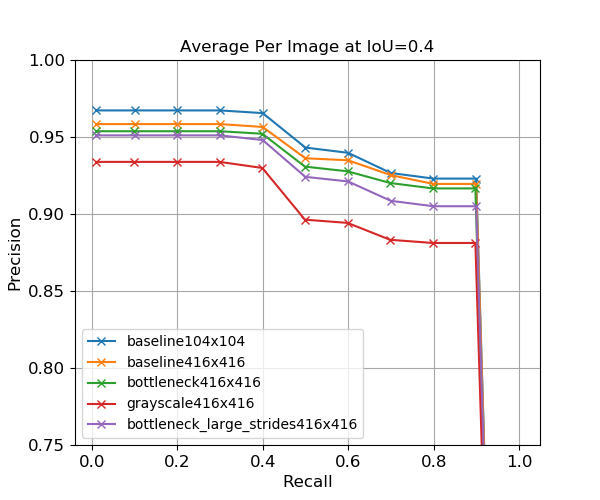
\includegraphics[width=\linewidth]{pr04}
	\caption{Average Precision Recall in terms of bounding boxes over 1000 images with about 1.3 gates per image. That is Precision Recall is calculated for each image, then interpolated and averaged.}
	\end{minipage}
\hfill
\begin{minipage}{0.45\textwidth}
	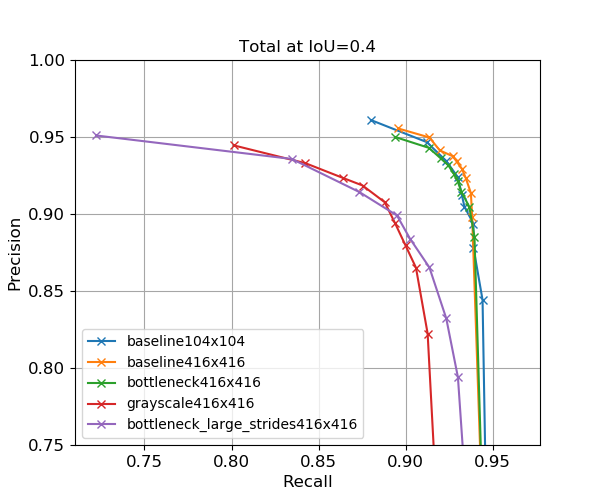
\includegraphics[width=\linewidth]{totalpr04}
	\caption{Total Precision Recall in bounding boxes over 1000 images with 1372 boxes in total. }
\end{minipage}
\label{fig:pr}
\end{figure}

\section{Bounding Box Accuracy}

A general problem I met is the accuracy of the predicted bounding boxes. Fig. \ref{fig:area} shows average precision for different box sizes. We see how the model is significantly better at smaller boxes. The reason could lay in the imbalance in the training set, Fig. \ref{fig:hist} shows a histogram of bounding box sizes. A similar distribution is present in the test set.

When we look at the performance for different iou thresholds Fig. \ref{fig:iou}, we see how well the bounding boxes fit. All models drop in similar fashion with higher ious. One could have expected that models with higher resolutions are less affected but apparently this is not the case.

\begin{figure}[htbp]
	\centering
	\begin{minipage}{0.45\textwidth}
		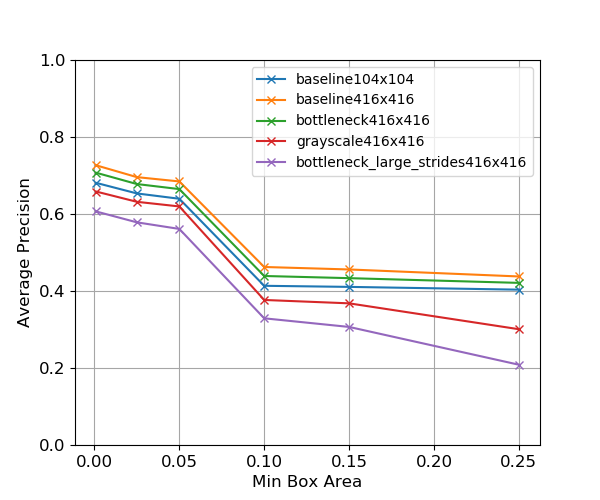
\includegraphics[width=\linewidth]{area}
		\label{fig:area}
		\caption{Average Precision for different sizes of bounding boxes (relative to image size). Each data point contains the range from where its drawn to the next data point. That is the first point contains the boxes with size 0.001 to 0.025.Average Precision is the average total precision at all recall levels.}
	\end{minipage}
\hfill
	\begin{minipage}{0.45\textwidth}
				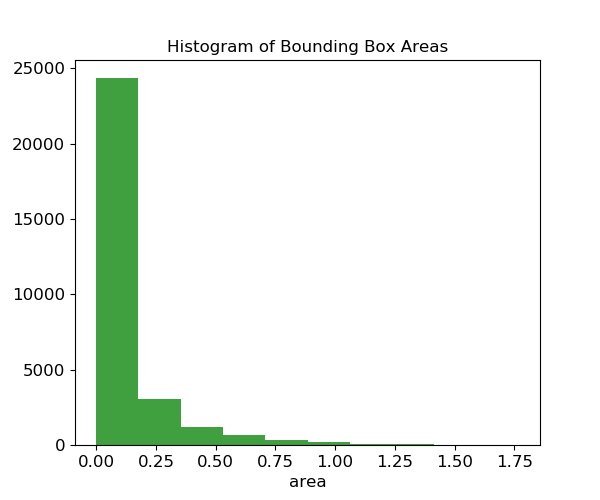
\includegraphics[width=\linewidth]{hist_training}
	\label{fig:hist}
	\caption{Bounding Box Sizes in the training set.}
	\end{minipage}

\end{figure}

\begin{figure}[htbp]

		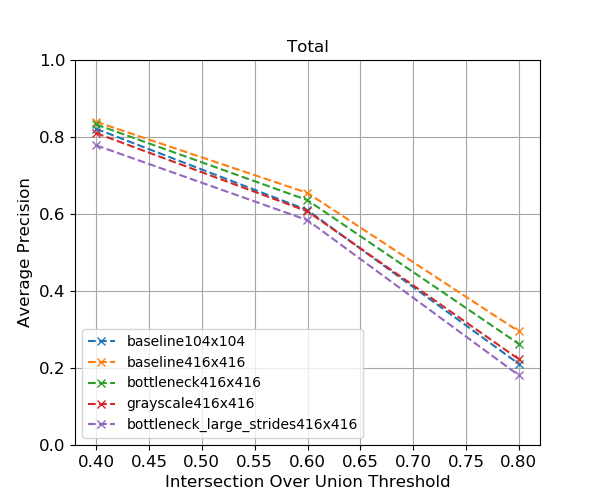
\includegraphics[width=0.5\linewidth]{iou}
		\label{fig:iou}
		\caption{Model Performance for different IoU levels. Average Precision is the average total precision at all recall levels.}
\end{figure}

\newpage


\section{Conclusion}
\begin{itemize}
	\item Using strides and bottlenecks should allow us to build a network that is fast enough.
	\item The bounding boxes are still too inaccurate. This does not really depend on the model size/resolution.
	\item There is quite an imbalance in performance between large and small boxes. This might be due to the distribution in the training set. 
\end{itemize}

\section{Next Steps}
\begin{itemize}
	\item Write it all down.
	\item Look for ways to refine bounding boxes.
	\item Create more large gates in training/test set.
\end{itemize}


\end{document}\grid
